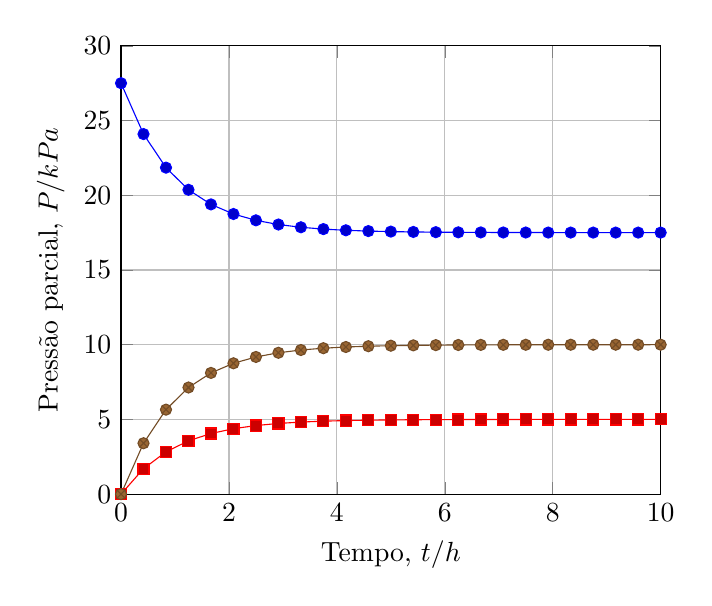
\begin{tikzpicture}
    \begin{axis}[
        xlabel={Tempo, $t/\unit{h}$},
        ylabel={Pressão parcial, $P/\unit{kPa}$},
        grid=both,
        ytick={0, 5, 10, 15, 20, 25, 30},
        xmin=0, xmax=10,
        ymin=0, ymax=30,
        domain = 0:10,
    ]
    \addplot {
        17.5 + 10*exp(-x)
    };
    \addplot {
        5*(1 - exp(-x))
    };
    \addplot {
        10*(1 - exp(-x))
    };
    \end{axis}
\end{tikzpicture}
